%\clearpage
\chapter{Etat de l'art}
\label{sec:SOTA}

Dans le cadre de cette thèse, nous cherchons dans un premier temps à lier la dynamique des articulations d'un piéton à une intention. Cette estimation de la dynamique des articulations sera ensuite combinée à la vision afin d’avoir une estimation plus robuste et absolue de l'intention du piéton en fonction de son environnement.\\

L'idée de restreindre la gestuelle d'une personne à la seule dynamique de son ossature n'est pas nouvelle.
Durant les années 70, les travaux en psychologie de Johansson  \cite{johansson1973visual,johansson1976spatio} ont permis de montrer qu'avec seulement des points lumineux, l'être humain interprétait facilement les stimulis qui lui étaient présentés comme ceux d'un être humain effectuant des actions: l'humain peut donc reconnaitre une action juste avec la pose et sans information annexe telle que l'environnement. 

De ce fait, nous avons souhaité voir s'il était possible de réaliser l'analogie entre les travaux réalisés sur le stimuli humain et la machine.

\begin{figure}[H]
    \centering
    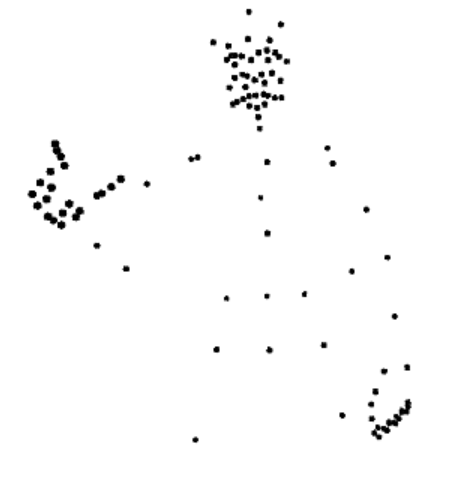
\includegraphics[width=0.34\linewidth]{Images/Johansson.png}
    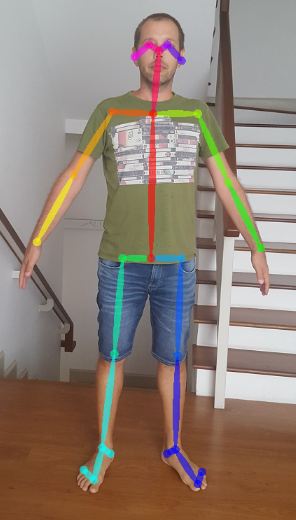
\includegraphics[width=0.2\linewidth]{Images/openpose2.png}
    \caption{A gauche: Un exemple de stimuli de l'experience de Johansson \cite{johansson1973visual,johansson1976spatio}.\\ A droite: la squelettisation obtenue après l'application d'Openpose \cite{cao2017realtime}}
    \label{fig:Johansson}
\end{figure}

Par conséquent, nous 

\textit{De ce fait, nous avons du nous intérésser à plusieurs étapes qui seront considérées comme des parties indépendantes de notre approche}


PipeLine: SQUELETTE -> HAR -> INTENTION

\section{Squelettisation de piétons}
La nécéssité première de cette thèse consiste donc en l'obtention d'une squelettisation cohérente de chaque piéton présent dans l'image au fil du temps.

Cette squelettisation sera ensuite utilisée en tant que donnée d'entrée de notre réseau afin d'en inférer une classe en fonction de la gestuelle de celui-ci.

La tâche de détection est compliquée par la variabilité de l’apparence des personnes (vêtements, pose ...)
ainsi que par des phénomènes d’occlusions, dûs à la foule et au décor ou encore dûs à des problèmes d'echelle dans l'image.




\label{subsec:SQUEL}
\subsection{Approches Top Down}
\subsection{Approches Bottom Up}

\section{Human Action Recognition}
\label{subsec:HAR}

La seconde étape de l'approche consistera en la classification des actions de la personne. La reconnaissance de l'action humaine dans une vidéo est un sujet de recherche difficile de par la grande variation et la complexité des données en entrée.

Les principales modalités utilisées pour la reconnaissance d'actions humaines comprennent les vidéos RGB dans leur intégralité \cite{donahue2015long,2014arXiv1412.0767T,varol2017long,Wu_2018_CVPR}, le flow optique \cite{simonyan2014two,zhang2016real,sevilla2018integration,DanutPOP} et la réprésentation sous forme de squelette \cite{vemulapalli2014human,du2015hierarchical,2016arXiv160707043L,2018arXiv180107455Y}.

Selon notre problématique: lier la dynamique de la pose à une classe, nous nous sommes majoritairement intéréssés à la dernière famille d'approches. La représentation sous forme de squelette qui semble être l'approche la plus robuste mais également la plus plausible pour une utilisation en temps réel:

\begin{itemize}
    \item En réduisant la taille des données d'entrée grâce à la structure de données associée aux squelettes, ce type d'approche est considéré comme bien plus rapide computationellement parlant que les modalitées listées précédement.
    \item Par ailleurs, celles-ci sont généralement bien plus robustes et capables de représenter les informations invarriantes d'une action puisque qu'aucun contexte de fond n'y est inclus.
\end{itemize}



\subsection{Sequence based}

Ces dernières années, les réseaux de neurones récurrents ont  été les approches de référence pour la modélisation de séquences en matière de reconnaissance vocale, de traitement numérique des signaux, de traitement vidéo et d'analyse des données textuelles. La plupart des approches d'apprentissage profond pour la reconnaissance de gestes utilisent des cellules récurrentes comme les LSTM \cite{hochreiter1997long} ou les GRU \cite{2014arXiv1406.1078C}.

On représente le squelette sous forme d’une séquence et on y applique des réseaux de neurones à état, permettant de conserver l’information d’un instant de la séquence à un autre.



\subsection{Image-Based}
Les cellules récurrentes sont relativement lentes et difficiles à entrainer ainsi qu'à utiliser en temps réel comparé aux approches dites convolutives.

Les approches Image-Based peuvent par exemple représenter le squelette sous la forme d'une pseudo-image pour appliquer des réseaux de convolutions, ou tout autre version spatio-temporelle des CNN.

L’idée étant d’utiliser la connaissance du domaine image qui s’est améliorée ces dernière années et de structurer les données pour leur donner la forme escomptée (une suite d’image) et enfin réaliser une classification habituelle.


En s'éloignant un peu plus du domaine image mais en conservant la dimension convolutive, d'autres approches à base de CNN, les utilisent en tant que CNN 1D:

Les réseaux récurrents et les réseaux convolutifs peuvent également être fusionnés. L'approche consiste à extraire les caractéristiques avec des couches convolutives, adaptées pour exploiter les informations spatiales, puis de modéliser la dynamique temporelle par des couches récurrentes.

Ainsi, Li et al.(2017)\cite{li2017skeleton} proposent une approche où LSTM et CNN sont fusionnés "tardivement" (late fusion). Ullah et al.(2017)\cite{ullah2017action} proposent un approche bidirectionnelle où, les features obtenus par le CNN sont envoyés dans un LSTM bidirectionnel \cite{Schuster97bidirectionalrecurrent}, connectant deux couches cachées de directions opposées à la même sortie. La couche de sortie pouvant alors obtenir simultanément des informations sur les états passés et futurs.



\subsection{Attention}

\subsection{Graph Based}

\section{Intention Prediction}
\textit{La plupart des approches actuelles de la prédiction de l'action des piétons sont basées sur la trajectoire [16, 1, 5], ce qui signifie qu'elles s'appuient sur le mouvement passé observé des piétons et/ou la dynamique des véhicules pour prédire l'emplacement futur des piétons. Ces approches sont toutefois efficaces lorsque les piétons traversent déjà laa rue ou sont sur le point de le faire, c'est-à-dire que ces algorithmes réagissent à une action déjà en cours au lieu de l'anticiper.}

Un remède aux inconvénients courants des algorithmes basés sur la trajectoire est d'anticiper l'action en estimant sa cause ou son intention non déviante.


In the literature various terms such as intention, actionand behavior are used to describe what the agent is doing or about to do in the scene. Here, we distinguish intention as the underlying state of mind which cannot be observed but can be inferred from the behavior. This is opposed toactions and, more generally, behaviors, i.e. observable ac-tions such as walking or crossing, for which there is groundtruth available.




\subsection{Handcrafted}
\subsection{Apprentissage profond}


